\documentclass[a4paper,notitlepage]{report}
\usepackage{url}
\usepackage{parskip}
\usepackage{graphicx}
\usepackage{float}
\usepackage{tikz}
\usepackage{circuitikz}
\usetikzlibrary{decorations.pathreplacing}
\usetikzlibrary{patterns}
\usepackage{listings}
\usepackage{color}
\definecolor{lightgray}{rgb}{.9,.9,.9}
\definecolor{darkgray}{rgb}{.4,.4,.4}
\definecolor{purple}{rgb}{0.65, 0.12, 0.82}
\lstdefinelanguage{JavaScript}{
  keywords={break, case, catch, continue, debugger, default, delete, do, else, false, finally, for, function, if, in, instanceof, new, null, return, switch, this, throw, true, try, typeof, var, void, while, with},
  morecomment=[l]{//},
  morecomment=[s]{/*}{*/},
  morestring=[b]',
  morestring=[b]",
  ndkeywords={class, export, boolean, throw, implements, import, this},
  keywordstyle=\color{blue}\bfseries,
  ndkeywordstyle=\color{darkgray}\bfseries,
  identifierstyle=\color{black},
  commentstyle=\color{purple}\ttfamily,
  stringstyle=\color{red}\ttfamily,
  sensitive=true
}

\lstset{
   language=JavaScript,
   backgroundcolor=\color{lightgray},
   extendedchars=true,
   basicstyle=\footnotesize\ttfamily,
   showstringspaces=false,
   showspaces=false,
   numbers=left,
   numberstyle=\footnotesize,
   numbersep=9pt,
   tabsize=2,
   breaklines=true,
   showtabs=false,
   captionpos=b
}

\begin{document}

\title{Logic Circuit Workbench: GatePlay}
\author{Greg O'Connor \\
		Computer Science, University of Oxford \\
		\\
		Third Year Project\\
		Supervisor: Geraint Jones}
\date{\today}
\maketitle

\begin{abstract}
GatePlay is an application to build and simulate logic circuits from within the web browser, without the need for installation or extra plug-ins. It is designed to couple a simple and aesthetically pleasing Graphical User Interface with an efficient and accurate simulation.
\end{abstract}
\clearpage

\tableofcontents
\clearpage

\chapter{Introduction}

\section{Motivation}
Logic circuits underpin practically every aspect of modern life in the form of computer chips. It is therefore important that people have the opportunity to learn about and understand logic circuits.

I believe that one of the best ways to learn about logic circuits is to build them, and that the most accessible way of doing that is by using a simulated workbench --- avoiding the cost and expertise required to build physical circuits. The workbench would not be designed to be used by professionals in designing chips, but for casual users looking to learn about logic circuitry.

Projects which attempt to solve the same problem can already be found on the Internet. Two of the best examples I could find were Logic.ly\footnote{http://logic.ly} and CircuitLab\footnote{http://www.circuitlab.com}.

Logic.ly was easy to use but had two major problems. First and foremost, the simulation implemented in Logic.ly over simplified: it does not assign any propagation delay to its components, making it difficult to see what happens in oscillating circuits. Secondly, it is implemented using Adobe Flash. Flash requires a web browser plug-in not included on many devices (notably iOS devices), which reduces Logic.ly's accessibility.

CircuitLab is designed more for power users and has a much steeper learning curve than Logic.ly. CircuitLab allows users to create general electronic circuits from power sources, resistors, etc. which adds to the complexity of the user interface. Even as someone who considers themselves computer literate, I found it difficult to use CircuitLab.

Therefore I decided to build a workbench which is easy to use but would not simplify the simulation more than necessary.

\section{Overview of GatePlay}
GatePlay can be seen in figure~\ref{fig:interface}. The labelled regions are:

\begin{itemize}
	\item[1] The \textbf{top bar}, which has buttons to download the workbench as an image and to start simulating the circuit. When simulating, the top bar has additional controls such as starting, restarting, and pausing the simulation
	\item[2] The \textbf{left bar}, which has sliding panels containing the  components available to build circuits with. The user simply drags a gate from the left bar onto the workbench to add it to the circuit
	\item[3] The \textbf{workbench}, which is where almost all interaction with GatePlay happens. When editing you can move, delete, and draw wires between components. When simulating wires are coloured to show their current value
\end{itemize}

The components and wires on the workbench snap to the grid lines which can be seen in the screenshots.

GatePlay has a library of standard components which can be used to build circuits. All of the components are implemented as black boxes, even though most of them can be re-implemented using a combination of the simpler components.

\begin{itemize}
	\item \textbf{Input} components such as constant $ON$, $Toggle$ (clicking on a $Toggle$ during simulation will change its value), and $Blinker$ (which flip their value at a constant interval)
	\item \textbf{Output} components such as $LED$s
	\item \textbf{Gates} implement standard boolean logic functions such as $NOT$, $AND$, and $XOR$
	\item \textbf{Function} components such half adders and full adders
	\item \textbf{Memory} components such as SR latches and D flip-flop  
\end{itemize}

A typical workflow for creating circuits would be:

\begin{enumerate}
	\item Drag the desired components from the left-bar on to the workbench
	\item Wire the components up by left-clicking on output ports, and then left-clicking on an input port. Fixed points can be created along the way by left-clicking on an empty part of the workbench
	\item Entering simulation mode by clicking on the ``Start Simulating'' button on the top-bar
	\item The simulation can now be paused, resumed, or advanced manually by using the controls in the top-bar
	\item The user may decide to return to editing mode to add, move, or delete components, or re-wire parts of the circuit
\end{enumerate}

Figure~\ref{fig:dflopflop} shows a D flip-flop being simulated on the workbench. Green wires are $True$ and red wires are $False$. The round components on the left are $Toggle$s; clicking them will change their value and cause the resulting changes to propagate through the circuit. The round components on the right are LEDs, which simply display their input value.

\begin{figure}[p]
    \centering
    \includegraphics[width=\textheight,angle=90]{labelled.png}
    \caption{Drawing a circuit}
    \label{fig:interface}
\end{figure}

\begin{figure}[p]
    \centering
    \includegraphics[width=\textheight,angle=90]{dflipflop.png}
    \caption{Simulating a D flip-flop}
    \label{fig:dflopflop}
\end{figure}
\clearpage
\chapter{Background}
\label{chapter:background}

\section{Logic Circuits}
\label{sec:circuits}
A \textit{k-ary Boolean function} is a function which $k$ boolean values and returns a boolean value.
\[ F : \{True, False\}^k \rightarrow \{True, False\} \]
\textit{Logic gates} are physical implementations of (typically simple) boolean functions. A \textit{logic circuit} is a collection of logic gates wired together, producing an implementation of a composition of boolean functions.

By composing ever more complex functions we can create physical implementations of useful circuits --- for example circuits which add or multiply numbers.

A gate has a \textit{propagation delay} defined as the time from when its inputs become stable and valid to when its outputs become stable and valid (cite wikipedia). Propagation delay changes based on the following factors

\section{Building Websites}
GatePlay is a web application. Instead of being installed on the user's computer it runs in their web browser. GatePlay is a single HTML document and has relatively few CSS style rules. The vast majority of the work was creating the JavaScript, which handles all interactions with the top and left bars, as well as displaying and editing circuits.

\begin{itemize}
	\item[HTML] defines the semantic structure of the website as a collection of nested elements, known as the DOM (Document Object Model) tree. In other words, HTML defines the content of a website and the structure of headings, sections, paragraphs, etc.
	
	\item[CSS] Cascading Style Sheets modify how HTML documents are displayed by the clients browser. CSS files are lists of \textit{selectors} with associated \textit{attributes}. A selector describes elements based on their position in the DOM tree, and its attributes modify how those elements are displayed. For example, it is easy to specify the following styles in CSS: ``All elements of type \textit{gate} should be 150 pixels wide'', or ``The middle section of the website should take up 80 percent of the width''.
	
	\item[JavaScript] JavaScript is a full programming language which is run in the user's browser when they load the website. It can perform arbitrary computations, and is also free to modify the DOM tree and the styles of elements.
\end{itemize}
\clearpage
\chapter{Requirements}
It was agreed that the project should satisfy the following requirements:

\begin{itemize}
	\item \textbf{Accessibility:} The workbench needs to be accessible to as many users as possible. This requirement is broken down into several sub-requirements:
	
		\begin{itemize}
			\item \textbf{Web based:} The workbench must be implemented in such a way that it is accessible from the Internet, and runs in the user's browser (rather than needing to be downloaded and installed) 
			
			\item \textbf{Plug-in free:} It should run in the browser without requiring third-party plug-ins such as Adobe Flash or Microsoft Silverlight. This effectively limits the implementation language to JavaScript or a language which is compiled to JavaScript.
			
			\item \textbf{Simple UI:} The user interface must be simple to understand and use. Users should be able to use familiar actions such as box selection, deletion using the Delete key, drag-and-drop, etc.
		\end{itemize}
	
	\item \textbf{Non-simplistic simulation:} While the workbench should be easy to use, it should not simply the simulation beyond what is reasonable. The simulation should take in to account the uncertainty in a gate's propagation delay.
\end{itemize}


\clearpage
\chapter{Simulation}
\label{chapter:simulation}

\section{Modelling Circuits}
A circuit can be modelled as a set of components and a set of wires. The fields which define components and wires are shown in figures \ref{fig:component} and \ref{fig:wire} respectively. The only constraint placed on circuits is that no more than one wire may go into the same input port of the same component.

\begin{figure}[H]
\centering
\begin{itemize}
	\item The \textbf{number of inputs} the component has ($N$)
	\item The \textbf{number of outputs} the component has ($M$)
	\item An \textbf{evaluation function} which takes a list of $N$ truth values and returns a list  of $M$ truth values
\end{itemize}
\caption{Fields of a Component}
\label{fig:component}
\end{figure}

\begin{figure}[H]
\centering
\begin{itemize}
	\item The \textbf{source component} which  the wire is leaving from
	\item The \textbf{output port} of the source component
	\item The \textbf{target component} which the wire is going to
	\item The \textbf{input port} of the target component
	\item The current \textbf{truth value} of the wire 
\end{itemize}
\caption{Fields of a Wire}
\label{fig:wire}
\end{figure}

We say that component $X$ is \textit{wired} to component $Y$ if there exists a wire $w$ in the set of wires such that $w$'s source component is $X$ and $w$'s target component is $Y$.

We assume for now that each component has a constant propagation delay $\delta$, which is defined by the component's evaluation function. The background section~\ref{sec:circuits} states that a gate's propagation delay actually varies, and we will take that into consideration later in this chapter.

\subsection{2-Valued Simulation}
Logic circuits are physical implementations of Boolean functions. The domain of Boolean variables is $\{True, False\}$, so a natural simulation would use the same two truth values for the evaluation functions in our model. In other words, each wire has one of two values: \textit{True} or \textit{False}. 

We consider the problems with a 2-valued simulation in section~\ref{sec:2-valued} and fix them by using a 3-valued simulation in section~\ref{sec:3-valued}, but for now let us set the domain of truth values to be $\{True, False\}$.

\section{Event-Based Simulation}
GatePlay uses an event-based algorithm to simulate logic circuits. An event is a notification that a specific output of a component has changed. They are defined by a 4-tuple $(X, P, T, V)$ where:

\begin{itemize}
	\item \textbf{X} is the \textbf{source component} the event is propagating from
	\item \textbf{P} is the \textbf{output port} on the source component which has changed value
	\item \textbf{T} is the \textbf{event time} at which it is occurring
	\item \textbf{V} is the new \textbf{truth value} of the output port
\end{itemize}

Events are stored in a priority queue, and have priority equal to their event time. Lower times are more urgent. 

\subsection{Initial Components}
\label{subsec:initial}
The first events in a simulation run are generated by what I call \textit{Initial Components}. An initial component is defined as a component which takes no inputs. Some examples of initial components are described below:

\begin{itemize}
	\item \textbf{Constant Components} such as $ON$ and $OFF$ never change value, and so place their events in the queue just once when the circuit is initialised
	
	\item \textbf{Timed Components} such as $Blinker$s toggle their output at a set interval. The algorithm to implement this is non-trivial and discussed in chapter~\ref{chapter:implementation}
	
	\item \textbf{External Components} such as $Toggle$s add events based on user interaction. Since the stimulus to create an event comes from outside the simulator, it is a simple case of putting a method to create circuit events in the circuit's public API
\end{itemize}


\subsection{The Event Loop}
The heart of an event-based simulation is the event loop which processes all the events and generates new events. The stages of the event loop body are shown in figure~\ref{fig:eventloop}.

\begin{figure}[H]
\begin{enumerate}
	\item \textbf{Fetch} the next event to be processed from priority queue
	\item \textbf{Update} the value of the wires connected to the event port
	\item \textbf{Recalculate} the output of any gates whose inputs changed
	\item \textbf{Propagate} the change by creating new events for each changed output
\end{enumerate}
\caption{Event Loop Body}
\label{fig:eventloop}
\end{figure}

\subsection{Event Loop Example}
Consider the circuit shown in figure~\ref{fig:simple}. Let $X$'s current output be $False$, the event queue contain a single event $ev = (X, 1, t, True)$, and the current time be $t$.

\begin{figure}[H]
\centering
\begin{circuitikz} \draw
	(1,0) node[not port] (not1) {}
	(3,0) node[not port] (not2) {}
	(not1.out) -- node[above] {A} (not2.in);
	\draw (not1) node[left=-2pt] {X};
	\draw (not2) node[left=-2pt] {Y};
\end{circuitikz}
\caption{Two $NOT$ Gates}
\label{fig:simple}
\end{figure}

When the event loop body executes at simulated time $t$, the following actions occur:

\begin{enumerate}
	\item Pop $ev$ from the queue
	\item Update $A$ --- the wire coming from $X$ port $1$ --- to be valued $True$
	\item $A$ enters $Y$, so $Y$'s input has changed. Apply $Y$'s evaluation function to the new input, which returns $False$ (as $\lnot True = False$)
	\item Since $Y$'s output changed, add the following new event to the queue: $(Y, 1, t + \delta, False)$ where $\delta$ is $Y$'s propagation delay
\end{enumerate}

As the event loop repeats, changes propagate through a circuit.

\subsection{Culling}
\label{subsec:culling}
Events can sometimes be discarded without being processed by the entire event loop body. For example, events which set an output port to the value it already is do not change anything in the circuit and can be discarded during stage 2 of the event loop.

\subsection{Event Race Conditions}
Consider the circuit shown in figure~\ref{fig:racecondition}:
\begin{figure}[H]
\centering
\begin{circuitikz} \draw
	(1,0) node[and port] (and1) {}
	(and1.in 1) node[anchor=east]{False - A}
	(and1.in 2) node[anchor=east]{False - B}
	(and1.out) node[anchor=west]{C - False};
	 \draw (and1) node[left=12pt] {Z};
\end{circuitikz}
\caption{AND gate}
\label{fig:racecondition}
\end{figure}

Let there be two events in the event queue: $ev_1 = (X, 1, t, True)$ and $ev_2 = (Y, 1, t, True)$ where wire $A$ leaves $X$ port $1$, and wire $B$ leaves $Y$ port $1$.  In other words, A and B both become $True$ at simulated time $t$. Now consider what happens in the event loop at time $t$.

Suppose we handle $ev_1$ first: We set $A$ to $True$, $B$ is still thought to be $False$, and therefore we add the event $ev_3 = (Z, 1, t + \delta, False)$ to the queue (as $True \land False = False$).

Next we handle $ev_2$: $B$ is set to $True$ and $A$ is known to be $True$, so we add the event $ev_4 = (Z, 1, t + \delta, True)$ to the queue (as $True \land True = True$).

The queue now contains two events with different truth values occurring on $Z$ port $1$ at the same time. At simulated time $t + \delta$, if $ev_3$ is handled first it will be culled and the circuit will be simulated correctly. However if it is handled second then the output of $Z$ will be calculated as $False$, despite both its inputs being $True$! Since we are using a priority queue and both events have the same priority, there is no defined behaviour for which event will be handled first.

The solution is to do a first pass through all events happening at time $t$ and update the values of each of the affected wires. We look at $ev_1$ at set $A$ to $True$, and at $ev_2$ and set $B$ to $True$. Now if we process $ev_1$: $A$ and $B$ are already set to $True$ because of the first pass, and we calculate $Z$'s output to be $True$. Handling $ev_2$ will again yield $True$, and one of the duplicate events will be culled.

There is a further refinement implemented in GatePlay: when we do the initial pass through all events happening at time $t$ we maintain a set  of the affected components. In this example both events only affect $Z$, so the set will be $\{Z\}$ --- sets do not store duplicate values. We then re-calculate the output of each component in the set and add the event to the queue. In this case, we will only calculate and add $(Z, 1, t + \delta, True)$ once.

\subsection{Efficiency}
The speed of an event-based simulation is proportional to the number of events being generated and processed. For this reason, reducing the time spend processing events through Culling (see section~\ref{subsec:culling}) is critically important.

Also note that (if sensible data structures are used) event-based simulations still perform well in circuits with a very large number of components and connections, so long as relatively few events are occurring. An efficient simulation is not necessary for GatePlay as the UI only allows users to build modest-sized circuits, but it is good to implement an efficient simulator regardless in case the UI is ever changed.

\section{Limitations of 2-Valued Simulations}
\label{sec:2-valued}

\subsection{Initialisation Values}
\label{subsec:2-valued initialisation}
In a 2-valued simulation all wires must be either $True$ or $False$ valued. It is necessary to initialise the wire values before the circuit begins, but what is a sensible default? Suppose we initialise all wires to $False$, and consider the circuit in figure~\ref{fig:initialisation}:

\begin{figure}[H]
\centering
\begin{circuitikz} \draw
	(1,0) node[not port] (not1) {}
	(not1.in) node[anchor=east] {False - A}
 	(not1.out) node[anchor=west] {B - False};
\end{circuitikz}
\caption{An inconsistently initialised $NOT$ Gate}
\label{fig:initialisation}
\end{figure}

To have both $A$ and $B$ both be initialised to be $False$ is inconsistent with the logic of a $NOT$ gate. The same would be true if wires were initialised to $True$. One option would be to add a boolean flag to wires indicating that no event has reach them yet and leave them uninitialised. GatePlay, however, fixes the problem by using a 3-valued simulation (section~\ref{sec:3-valued}).


\subsection{Propagation Delay Uncertainty}
\label{subsec:2-valued uncertainty}
As discussed in section~\ref{sec:circuits}, the \textit{Propagation Delay} of a component is the time it takes from its inputs being stable and valid to its outputs becoming stable and valid\cite{Wikipedia: Propagation Delay}. 

Previously we have assumed that this delay is constant for a given component, but in reality the precise delay varies based on temperature, voltage, and output capacitance\cite{Wikipedia: Propagation Delay}. Our model of logic circuits does not consider these factors and therefore cannot make an informed estimation of the true delay for each pass through a component.

We assume that the propagation delay is never less than $\delta_{min}$ and never greater than $\delta_{max}$. $\delta_{min}$ and $\delta_{max}$ can be different for different types of components.

\begin{figure}[H]
\centering
\begin{circuitikz} \draw
	(1,0) node[not port] (not1) {}
	(not1.in) node[anchor=east] {A}
 	(not1.out) node[anchor=west] {B};
\end{circuitikz}
\caption{A $NOT$ Gate}
\label{fig:2-valued-circuit}
\end{figure}

\begin{figure}[H]
\centering
	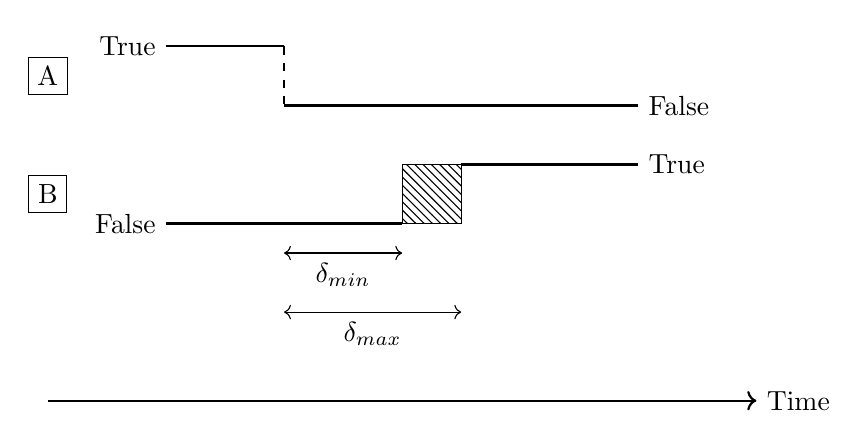
\begin{tikzpicture}[domain=0:4, xscale=1.5, yscale=0.75]
		\node[draw] at (-1,0.5) {A}; 
		\node[draw] at (-1,-1.5) {B}; 
   		\draw [thick] (0,1) node[left] {True} -- (1,1);
    	\draw [thick, dashed] (1,1) -- (1,0);
    	\draw [thick] (1,0) -- (4,0) node[right] {False};
    	\draw [thick] (0,-2) node[left] {False} -- (2,-2);
    	\draw [pattern=north west lines] (2,-2) rectangle (2.5,-1);
    	\draw [thick] (2.5,-1) -- (4,-1) node[right] {True};
    	\draw [thick,->] (-1,-5) -- (5,-5) node[right] {Time}; 
    	\draw [<->] (1,-2.5) -- (2,-2.5) 
			node [pos=0.5,anchor=north] {$\delta_{min}$};
		\draw [<->]	(1,-3.5) -- (2.5,-3.5) 
			node [pos=0.5,anchor=north] {$\delta_{max}$};
	\end{tikzpicture}
	\caption{Trace of a $NOT$ gate's input and output}
	\label{fig:2-valued-trace}
\end{figure}

Consider the circuit shown in figure~\ref{fig:2-valued-circuit}. If we flip A's value from $True$ to $False$ the trace of the truth values through time is shown in figure~\ref{fig:2-valued-trace}. $B$'s transition from $False$ to $True$ can happen at any point in hatched region based on the aforementioned factors. A 2-valued simulator at this level of detail can therefore only assume that the transition happens at a random time. In other words, the precise propagation delay for each pass through a component is randomly sampled from the interval $[\delta_{min}, \delta_{max}]$.

Each simulation of a circuit will likely have different propagation delays which can potentially change the output of a circuit altogether. If one run of this simulation yields a given result there is no guarantee that \textit{all} runs would yield the same result. I felt this was not desirable behaviour for a simulator. In the next section we introduce a simulator which models the uncertainly of components without introducing non-determinism in the simulation itself.

\section{3-Valued Simulation}
\label{sec:3-valued}
The way I decided to overcome the problems of 2-valued simulation described in section~\ref{sec:2-valued} was to instead use a 3-valued simulation. A wire has one of three values: $True$, $False$, or $Unknown$. A wire that is $Unknown$ is ``in reality'' either $True$ or $False$, but the simulation does not know which.

\subsection{Initialisation Values}
In a 3-valued simulation all wires can be initialised to $Unknown$ without the problem of inconsistency for 2-valued simulations discussed in section~\ref{subsec:2-valued initialisation}.

\subsection{Propagation Delay Uncertainty}
\label{subsec:3-valued uncertainty}
The 2-valued simulation was unable to model the uncertainty of component delay without making the result of each simulation run non-deterministic, as discussed in section~\ref{subsec:2-valued uncertainty}.

Suppose we have a component $X$ whose inputs are changing at time $t$. In the 2-valued simulation we would consider the outputs changing at time $t + \delta$ where $\delta$ is randomly sampled from the interval $[\delta_{min}, \delta_{max}]$. 

However in the 3-valued simulation we can consider the outputs of $X$ to be changing twice. At time $\delta_{min}$ they becoming $Unknown$, and then at time $\delta_{max}$ they settle on a stable value. 

By considering the output $Unknown$ for the duration of the delay uncertainty we have still modelled the uncertainty in the actual components, but without introducing uncertainty to our simulation. In other words, should a circuit yield a certain value in our simulation we know that it will yield the same value for \textit{all} possible combinations of gate delays.

Evaluation functions must also be augmented to accept $Unknown$ as in input, and potentially produce $Unknown$ as an output. For example, we define $True \land Unknown = Unknown$, $Unknown \land Unknown = Unknown$, and $False \land Unknown = False$.

\subsection{Event Suppression}
A bug was introduced in the simulator in section~\ref{subsec:3-valued uncertainty}. Consider the circuit shown in figure~\ref{fig:suppression}. Let $\delta_{min}$ and $\delta_{max}$ be the minimum and maximum gate delays respectively. $A$, $B$, and $C$ are all $False$.

\begin{figure}[H]
\centering
\begin{circuitikz} \draw
	(1,0) node[and port] (and1) {}
	(and1.in 1) node[anchor=east] {False - A}
	(and1.in 2) node[anchor=east] {False - B}
 	(and1.out) node[anchor=west] {C - False};
 	\draw (and1) node[left=12pt] {X};
\end{circuitikz}
\caption{An $AND$ Gate}
\label{fig:suppression}
\end{figure}

Let circuit event $e_1$ set $A$ to $True$ at time $t$, and event $e_2$ set $B$ to $True$ at time $t + 1$. It is now simulated time $t$. Using the algorithm thus far described we will handle $e_1$ and the following two events will be added to the queue: $e_3 = (X, 1, t + \delta_{min}, Unknown)$, $e_4 = (X, 1, t + \delta_{max}, False)$. Next, handling $e_2$ we will add the following events to the queue: $e_5 = (X, 1, t + 1 + \delta_{min}, Unknown)$, $e_6 = (X, 1, t + 1 + \delta_{max}, True)$.

The bug arises at simulated time $t + \delta_{max}$ when we handle $e_4$. At that time $C$ is set to $Unknown$ and we will set it to $False$. However this is incorrect behaviour as $e_2$ means that $C$ should be uncertain until $e_6$ is handled at time $t + 1 + \delta_{max}$.

In other words, the output of X is uncertain for two distinct reasons. $e_1$ causes $C$ to be uncertain in the interval $[t + \delta_{min}, t + \delta_{max})$, and $e_2$ makes $C$ uncertain in the interval $[t + 1 +  \delta_{min}, t + 1 + \delta_{max})$.

The simulator therefore must keep track of the intervals a wire is uncertain for, and \textit{suppress} any events which try to set it to a certain value in any of those intervals. In this example $e_4$ must be suppressed.
\clearpage
\chapter{Implementation}
\subsection{Loading Javascript and Require.js}
When the GatePlay site is visited, the only file downloaded is the main HTML file: index.html. The index then directs the user's browser to download the additional CSS and JavaScript files needed to run GatePlay.

JavaScript files are imported into a webpage using the Script tag. For a file to be correctly loaded all of its dependencies must have been run already.

\begin{figure}
\begin{lstlisting}[language=html]
...
<!-- componentview depends on component, so we ensure component is loaded first -->
<script type="text/javascript" src=".../component.js"></script>
<script type="text/javascript" src=".../componentview.js"></script>
...
\end{lstlisting}
\caption{}
\end{figure}

However it is time consuming for a human to find and type out a correct ordering for the imports, and would potentially need to be updated every time a file as added or modified.

Require.js is a JavaScript file loader which does this automatically. Each JavaScript file declares each of its direct dependencies, and Require.js will ensure they are all loaded correctly when the webpage loads.

\begin{lstlisting}[language=JavaScript]
// componentview.js

require([
	// Declare the path of each file we require	
	"canvas/model/component".
], function(Component) {
	// Each included file is run, and we can give a name to whatever it returns if desired
	var myComponent = new Component();
	...
});
\end{lstlisting}

\subsection{jQuery}
Different browsers provide subtly different ways for JavaScript to interact with the DOM tree - making multi-browser compatible code tedious to write and maintain.

jQuery is a ubiquitous JavaScript library which provides a single API for common JavaScript actions across many versions of different browsers:

\begin{lstlisting}[language=JavaScript]
require([
	"lib/jquery".
], function($) {
	// Select elements which are of class "gate"
	var gateElements = $(".gate");
	
	// Set the width of each gate to 100px
	$(gateElements).each(function() {
		$(this).width("100px");
	});
});
\end{lstlisting}

\section{Canvas}
GatePlay's main canvas is where we view and edit circuits. It is an HTML Canvas element, which


\subsection{Fabric.js}
HTML Canvas elements provide only low level drawing tools. You are able to draw shapes and images on them, but there is no concept of persist objects on the canvas.

Fabric.js is a library which wraps HTML Canvases with an object model, allowing GatePlay to interact at the level of objects being added to, modified, and remove from the canvas. 

Suppose I wanted to add a rectangle to a canvas, and then move it to a new location. Using Fabric.js this is two library calls (one to add a rectangle object and one to change the position property of the object). Using an HTML Canvas it is still one call to draw the rectangle, but moving it would require calculating is behind the rectangle, drawing that over the rectangle, and then re-drawing the rectangle at its new location.

Initially GatePlay used a different canvas framework called KineticJS but at the time the API documentation was not as good and so I transitioned to using Fabric.js.

\section{Simulator}
GatePlay's simulation is a plain JavaScript implementation of the concepts explained in 

\subsection{TruthValue}


\subsection{Component}
A component is defined by the following class constructor:

\begin{lstlisting}[language=JavaScript]
function Component(id, funcId, inputCount, outputCount, cArg) {
    this._id = id;
    this._funcId = funcId;
    this._inputCount = inputCount;
    this._outputCount = outputCount;
    this._cArg = cArg;

    this._evalFunc = Functions.get(funcId, cArg);
}
\end{lstlisting}

\begin{itemize}
	\item[id] \hfill \\ 
	Is the unique identifier of this instance of a component. It is provided as a parameter in the constructor because it is simpler to use the same id for the object drawn on the canvas and the Component in the simulation.
	\item[funcId] \hfill \\ 
	This is the id of the evaluation function of the Component. For example an AND gate would have funcId being "and".
	\item[inputCount]
	\item[outputCount]
	\item[cArg] \hfill \\ 
	An optional parameter for gates which require it. For "blinker" components cArg is set to the period of the blinker. For simpler components like "and" it is unset.
	\item[evalFunc] \hfill \\ 
	We fetch the appropriate evaluation function from the function store
\end{itemize}

\subsection{Evaluation Functions}
An evaluation function is first defined by the abstract class EvaluationFunction. It provides code common to all Evaluation Functions, such as checking that the list provided to the function "evaluate" is of a suitable size.

\begin{lstlisting}[language=JavaScript]
// Define the class with two parameters
function EvaluationFunction(minInputCount, maxInputCount) {
    this._minInputCount = minInputCount;
    this._maxInputCount = maxInputCount;
}

// Define "evaluate" function
EvaluationFunction.prototype.evaluate = function(argList, clock) {
    if (typeof argList == "undefined" || !argList instanceof Array)
        throw "argList must be a list";

    if (argList.length < this._minInputCount || argList.length > this._maxInputCount)
        throw "Invalid number of arguments passed to EvaluationFunction";

    return this._doEvaluate(argList, clock);
};

// "_doEvaluate" must be overridden by subclasses of EvaluationFunction
EvaluationFunction.prototype._doEvaluate = function(argList, clock) {
    throw "_doEvaluate not implemented on EvaluationFunction, you must override it";
}

// Default gate delay is 5 clock cycles
EvaluationFunction.prototype.getDelay = function() {
    return 5;
}

// Default uncertainty duration is 1 clock cycle
EvaluationFunction.prototype.getUncertaintyDuration = function() {
    return 1;
}
\end{lstlisting}

Individual implementations of evaluation functions then inherit from EvaluationFunction.

\begin{lstlisting}[language=JavaScript]
	// Define the "And" class
    function And() {
    }
    
    // Inherit from EvaluationFunction
    // We define that an And gate must have at least two inputs, but there is no upper bound (we can simulate n-input AND gates)
    And.prototype = new EvaluationFunction(2);
    
    // Provide an implementation for "_doEvaluate"
    And.prototype._doEvaluate = function(argList, clock) {
        var onlyTrue = true;

        for (var i = 0; i < argList.length; i++) {
            var v = argList[i];
            
            // If any of the arguments are FALSE, return FALSE
            if (v === TruthValue.FALSE) {
                return [TruthValue.FALSE];
            }
            onlyTrue = onlyTrue && v === TruthValue.TRUE;
        }
		
		// If all values are TRUE, return TRUE
        if (onlyTrue) {
            return [TruthValue.TRUE];
        
		// Otherwise we have zero FALSE values and at least one UNKNOWN value, so the output is UNKNOWN        
        } else { 
            return [TruthValue.UNKNOWN];
        }
    };
\end{lstlisting}

Because our implementation of the And function does not override the "getDelay" and "getUncertaintyDuration" functions, it has the default values of 5 and 1 respectively.

\subsection{Wire}
Wires are defined as follows for the simulation

\begin{lstlisting}[language=JavaScript]
define([
    "sim/truthvalue"
], function(TruthValue) {
    function Wire(id, sourceId, sourcePort, destId, destPort) {
		// Wire id    
        this.id = id;
        
        // Id of source component
        this.sourceId = sourceId;
        
        // Output index from the source component
        this.sourcePort = sourcePort;
        
        // Id of the destination component
        this.destId = destId;
        
        // Input index to the destination component
        this.destPort = destPort;
        
        // Current truth value of the wire (starts as UNKNOWN)
        this.truthValue = TruthValue.UNKNOWN;
        
        this.unstableUntil = 0;
    }

    return Wire;
});
\end{lstlisting}

\subsection{application.js}
\clearpage
\chapter{Testing}

\section{Unit Testing}

\section{Test Circuits}
\clearpage
\chapter{Conclusions}
Evaluating GatePlay against each of the requirements stated in chapter~\ref{chapter:requirements} I reach the following conclusions:

\paragraph{Accessibility}
GatePlay runs in all modern web browsers without the need for plug-ins, and satisfies those aspects of the requirements. The feedback I received from those who saw GatePlay running was that the user interface was appealing and simple to use. Some people found the workflow for creating wires slightly unintuitive (you single click to start drawing, rather than click and hold), so a miniature tutorial to guide new users through the interface would certainly be of benefit.

\paragraph{Simulation}
I am pleased with the level of simulation implemented in GatePlay. Having gate propagation delays allows users to see clearly how changes in the inputs to a circuit propagate through to the outputs. I am also satisfied that users of GatePlay will not come away with an over-simplified view of logic circuits which might harm their understanding in the future.

\subsection{Future Work}
While I am very pleased with GatePlay as it is today, there are some features that would improve it further.

\subsubsection{Wires over components}
It was always my intention that wires should be able to cross each other, but not cross over components. The workbench Circuit model is able to check if wires cross over any components, but the handler code for moving components became extremely complicated when it had to account for the position of wires. Ultimately I did not resolve the issue, and wires can travel over components.

\subsubsection{Moving wires when components are moved}
When a component is moved, all the wires to and from that component are deleted. I considered two other strategies for preserving the wires: either creating fixed points where the component ports used to be, or using A* search to find a new path for each wire. In the end I implemented neither. In the future I would like to implement a better strategy for moving wires when a component moves. 

\subsubsection{Saving circuits as black-boxes}
I useful feature would be the ability to create circuits and then save them for use as a black-box later. GatePlay has an existing notion of inputs ($Toggle$s) and outputs ($LED$s) and it would not be much more work to allow users to ``compile'' their workbench to a black-box.

\subsubsection{Simulation oscilloscope}
The circuit simulator emits a stream of wire value changes as it runs. In GatePlay, these are handled by the Application class and used to colour the wires on the workbench. In addition to this, it would be useful to be able to view traces of the wire values through time, and I would have liked to write a module to create such traces.
\clearpage
\begin{thebibliography}{9}

\bibitem{logicly} http://logic.ly.

\end{thebibliography}

\end{document}